\chapter{Resultados e Discussão}

O presente capítulo contém os resultados obtidos pelo ponto de vista do autor e da associação. Também serão apresentadas as dificuldades encontradas durante o processo de implementação do portal e do sistema de associados, desde a configuração e utilização de uma VPS até problemas encontrados nas ferramentas utilizadas. Também é neste capítulo que algumas telas de ambas aplicações ficarão disponíveis, tanto na visão de um visitante quanto na visão de um administrador.

\hspace{2.5cm}
\section{Apresentação das telas}
\label{subsec:telas}
\hspace{2.5cm}

Na presente seção estão as figuras demonstrativas do portal e do sistema gerencial. Por existirem diversas telas em ambos sistemas, só serão apresentadas as telas de autenticação de usuário e iniciais dos mesmos.

A primeira tela, representada na Figura \ref{fig:login-portal}, exibe a tela de autenticação do portal. Para gerenciar todo e qualquer conteúdo neste é necessário ter um cadastro com níveis de permissão suficientes para tal e inserir nome de usuário e senha nos campos correspondentes.

\begin{figure}[htb]
 \centering
 \caption{Página de login do portal}
 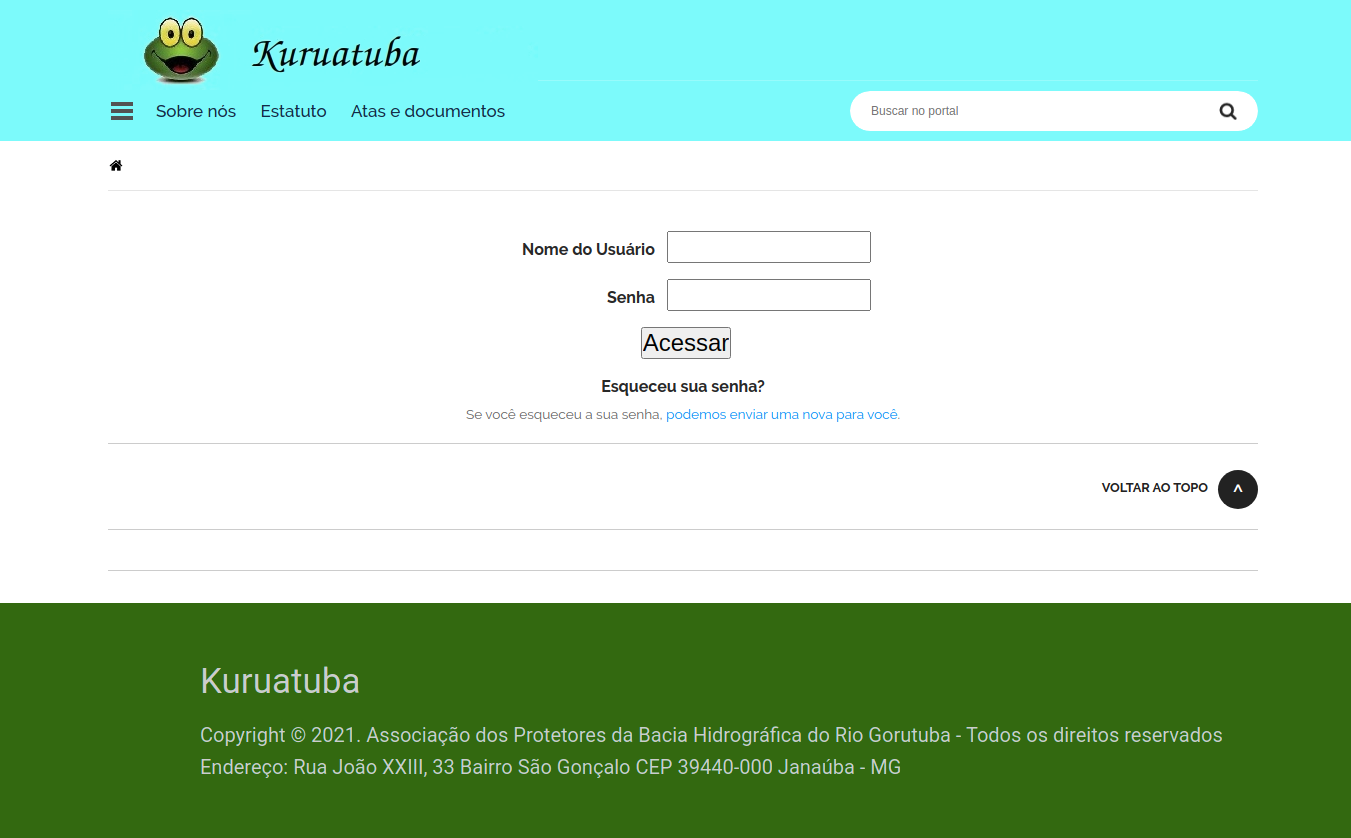
\includegraphics[width=1\textwidth]{figuras/kuruatuba_portal_login.png}
 \fonte{Autor.}
 \label{fig:login-portal}
\end{figure}


A Figura \ref{fig:home-portal} apresenta a página inicial do portal da Kuruatuba. Todo o conteúdo da página está disponível a qualquer pessoa para acesso e é alterado com menos frequência que outras páginas, com excessão das áreas reservadas a notícias e eventos.

\clearpage
\newpage

\begin{figure}[htb]
 \centering
 \caption{Página inicial do portal}
 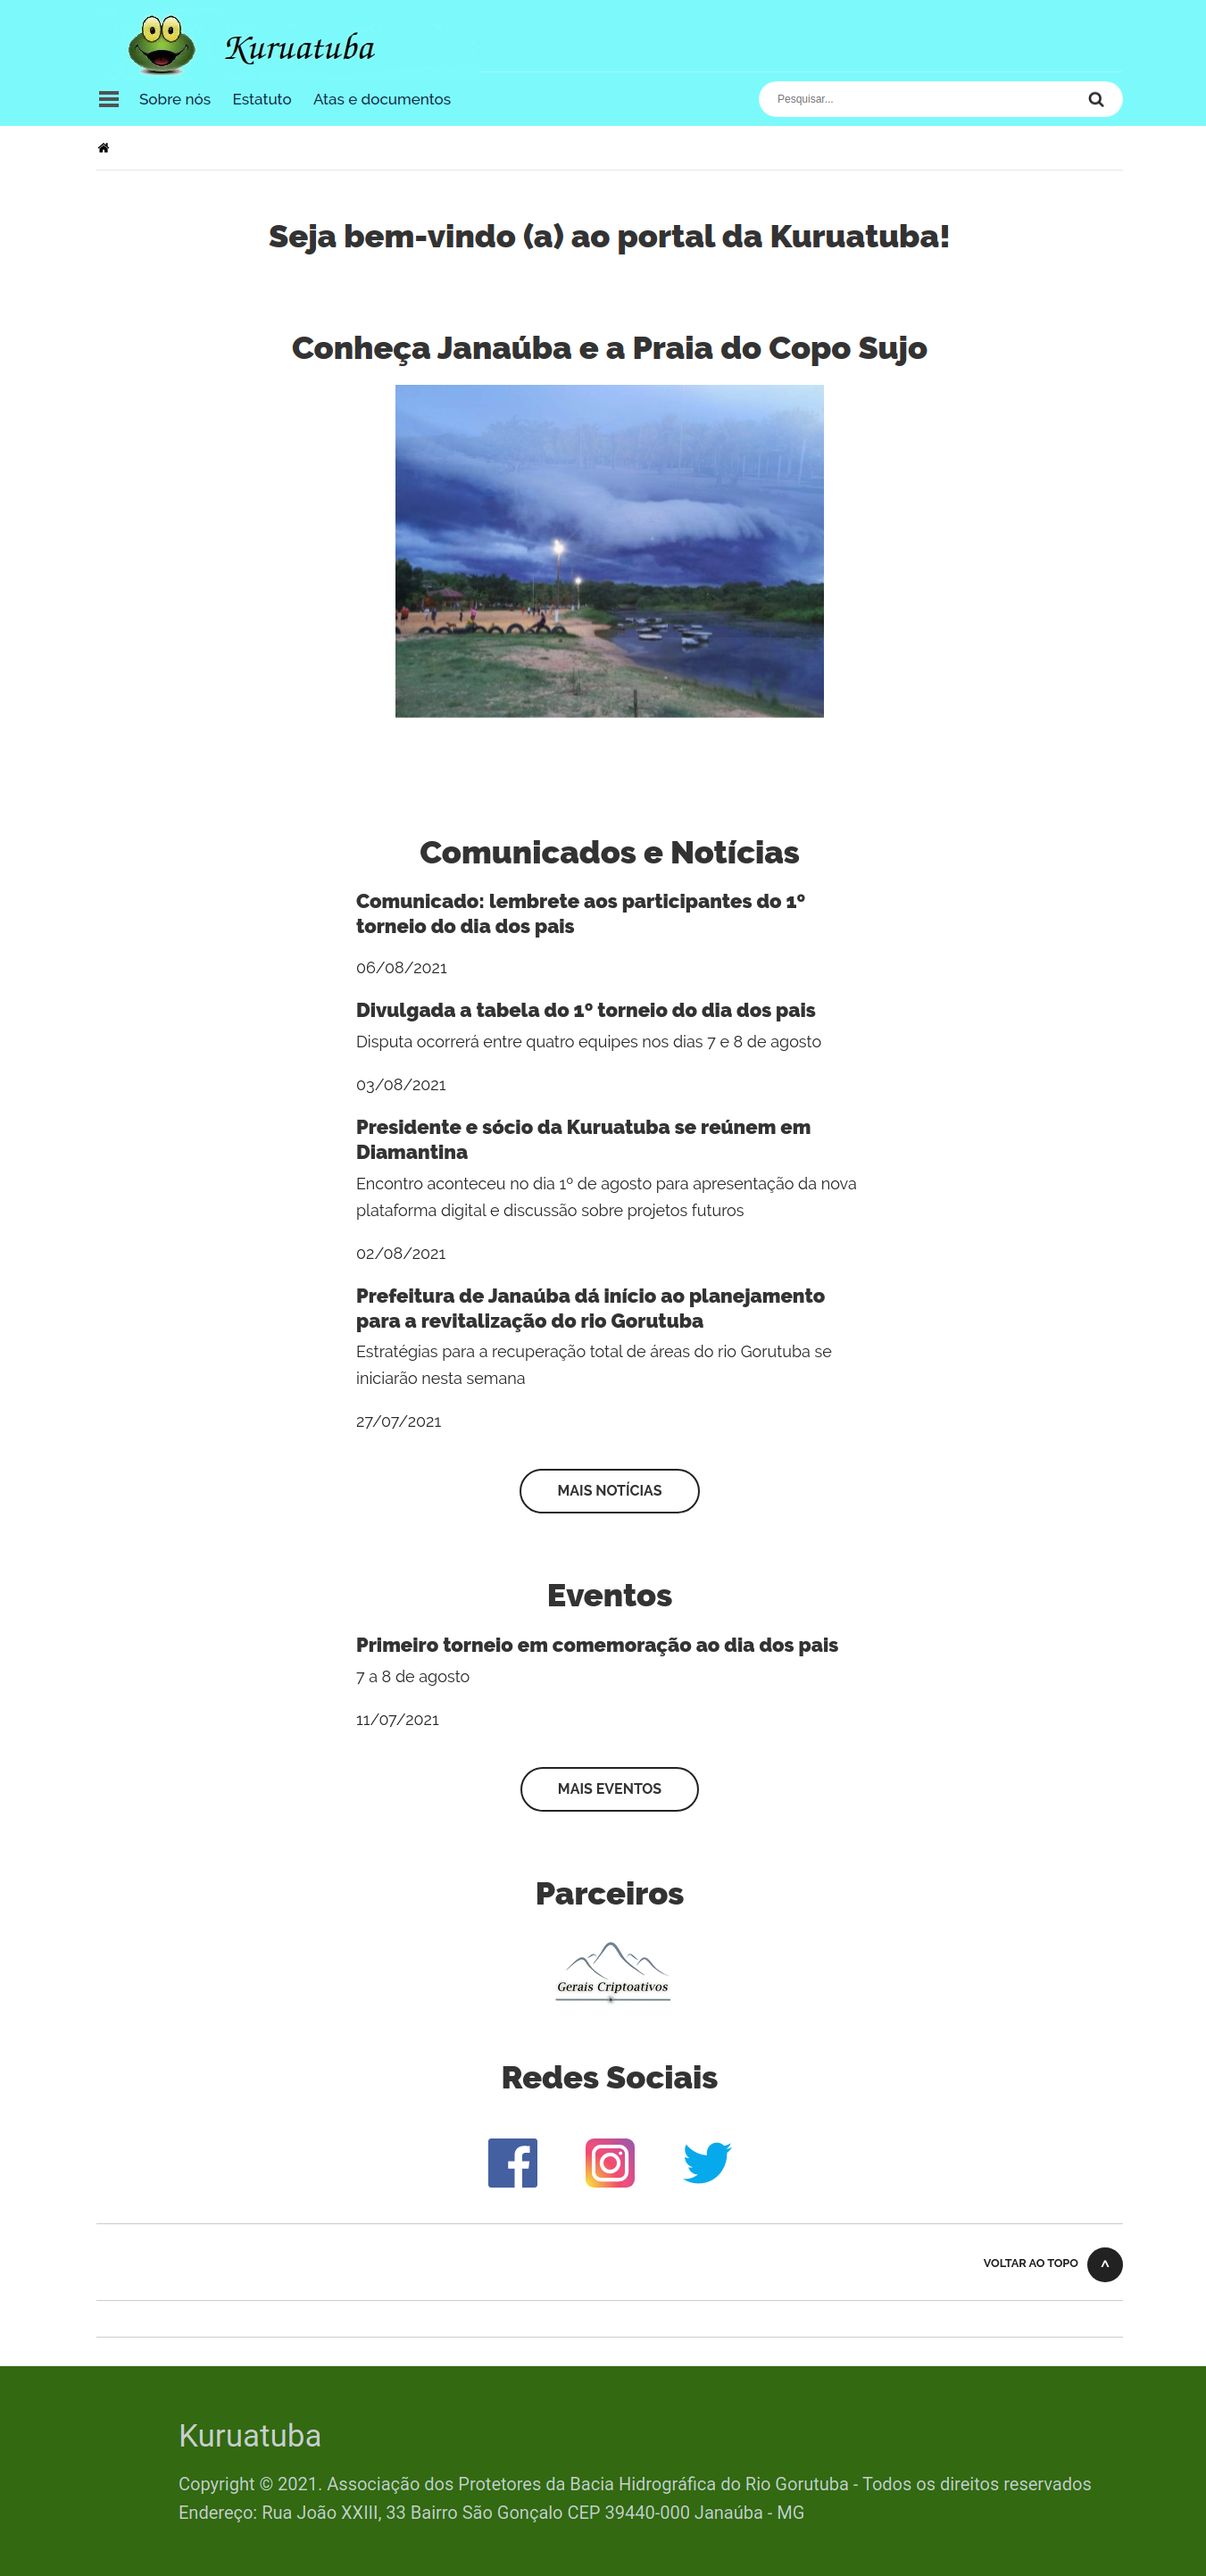
\includegraphics[width=0.7\textwidth]{figuras/kuruatuba_portal_home.png}
 \fonte{Autor.}
 \label{fig:home-portal}
\end{figure}

\newpage
\clearpage

A tela de autenticação do sistema de associados está apresentada por meio da Figura \ref{fig:login-sistema}. Convém mencionar que a opção de menu ``Administradores'' é exibida ao passar o cursor do \textit{mouse} sobre o botão ``Associados'', simulando um efeito típico de menus \textit{dropdown}. Para capturar tal opção, a captura da tela foi executava com o efeito \textit{hover} do CSS ativado na página pelo navegador. 


\begin{figure}[htb]
 \centering
 \caption{Página de login do sistema de associados}
 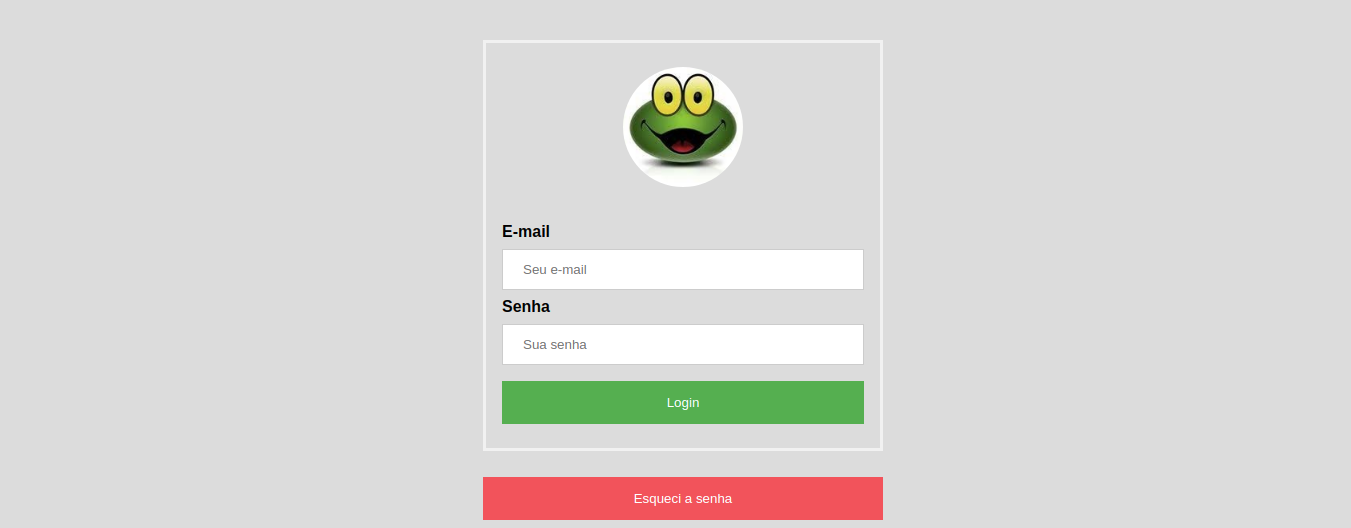
\includegraphics[width=1\textwidth]{figuras/kuruatuba_sistema_login.png}
 \fonte{Autor.}
 \label{fig:login-sistema}
\end{figure}


A tela inicial do sistema está representada na Figura \ref{fig:home-sistema}. Essa é a primeira página após a autenticação do usuário realizada na Figura \ref{fig:login-sistema} e os dados de associados exibidos são completamente fictícios, apenas exemplificam como  os dados reais estarão dispostos na tela para o usuário.

\newpage

\begin{figure}[htb]
 \centering
 \caption{Página inicial do sistema de associados}
 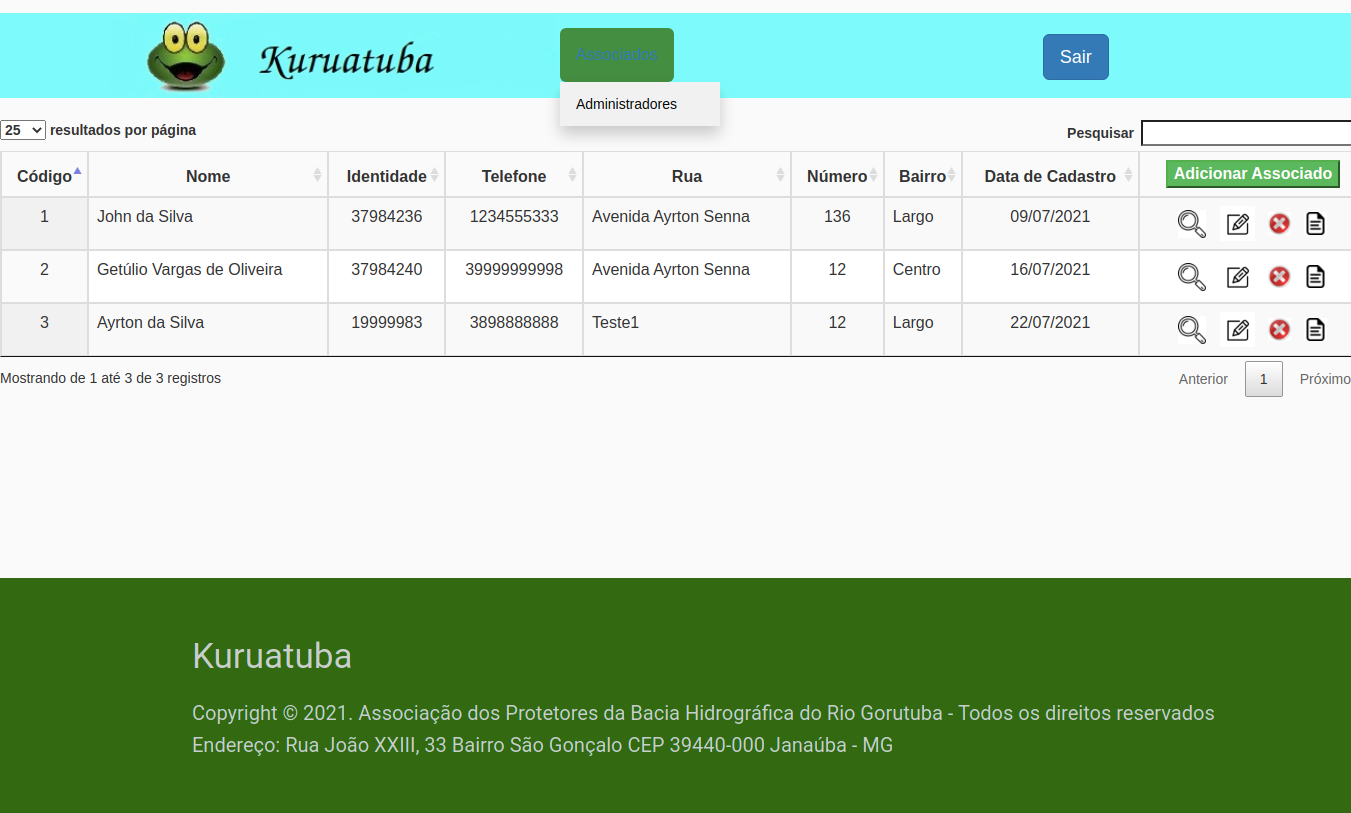
\includegraphics[width=1\textwidth]{figuras/kuruatuba_sistema_home.png}
 \fonte{Autor.}
 \label{fig:home-sistema}
\end{figure}


\clearpage

\hspace{2.5cm}
\section{Discussão}
\hspace{2.5cm}

Durante a execução do projeto algumas dificuldades foram enfrentadas, tanto em termos técnicos quanto em relação à comunicação com o cliente. No que concerne à comunicação, é fundamental ressaltar que as adversidades não se iniciaram desde a coleta de requisitos, como é recorrente em diversos outros trabalhos, mas sim durante a criação das páginas do portal, período em que o desenvolvedor necessita estipular um prazo relativamente grande para conseguir finalizar a publicação dos conteúdos.

Houve grande dificuldade em receber as informações necessárias para as páginas dos projetos sociais e para a inicial, sendo esta a de maior importância por ser a responsável por estabelecer o primeiro contato entre o visitante e o sistema. Também existiu impasse na escolha de quais imagens inserir na galeria da associação, visto que foi grande o número de arquivos recebidos e filtrar quais poderiam ser disponibilizados publicamente, além de verificar a existência de imagens iguais, foi um processo desgastante.

Tais obstáculos se somam aos encontrados quando se desempenha os papéis do \textit{Scrum}. Ser capaz de verificar junto ao cliente as dependências e as funcionalidade já criadas, implementar os requisitos a nível técnico e identificar problemas que podem estar influenciando no desenvolvimento do projeto são atribuições complexas que exigem muito de seus representantes, sobretudo quando é somente um responsável, e do cliente, pois ele deve estar ciente de tais limitações e ser capaz de entender as dificuldades relatadas pelo encarregado de construir o que foi combinado.

Se tratando das ferramentas e das tecnologias manuseadas, surgiram dúvidas ao configurar o apontamento do domínio contratado para a hospedagem principalmente por dois motivos: a inexperiência do desenvolvedor em realizar tal tarefa e o fato de duas empresas estarem fornecendo o domínio e a hospedagem, já que possuem diferentes responsabilidades e plataformas de gerenciamento. Porém foi possível sanar todas as dúvidas através do suporte on-line dos fornecedores.

Todas as adversidades citadas anteriormente impactam diretamente nos prazos das entregas, estimulando sua prorrogação e dificultando o seguimento das atividades. Embora tenha ocorrido, o adiamento de entregas foi minimizado graças à adoção de uma metodologia ágil e do total comprometimento com o projeto. Juntamente com os aspectos mencionados, o grande entendimento sobre os objetivos da associação e sobre grande parte das ferramentas utilizadas também foi importante para o cumprimento dos prazos e para a satisfação do cliente.

Abordando agora aspectos voltados para a segurança do produto, torna-se necessário distinguir o portal do sistema gerencial de associados, visto que para o primeiro foi utilizado um CMS de grande potencial nesse quesito, conforme está representado na Figura \ref{plone}, enquanto para o segundo não houve utilização de algum \textit{framework} ou gerenciador de conteúdo. 

Portanto, as principais medidas implementadas pelo desenvolvedor quanto à segurança das informações foram adicionadas ao sistema de associados, que focam em impedir ou dificultar não só ataques relacionados a SQL \textit{Injection} e sequestro de sessão \footnote{Tipos de ataque cibernéticos comumente aplicados em sistemas web. Saiba mais em: \citeonline{netomitigando}.}, como também inconsistências que possam ser geradas pelo próprio usuário, como: duplicidade de registros em banco de dados, cadastro de informações pessoais inválidas e exclusão involuntária ou logicamente não permitida segundo às regras de negócio da associação.

Por fim, ressaltando os beneficios proporcionados à associação através da utilização do novo sistema de informação, houve um ganho no alcance das publicações através de sua divulgação entre colaboradores e registrado pelo \textit{Google Analytics}, que, por sua vez, registrou a visita de mais de 40 visitantes após seu lançamento, oriundos de diferentes localidades. Demais ganhos são inquestionáveis e compreendem desde a intuitividade em acessar e gerenciar conteúdos digitais até a segurança e disponibilidade de dados confidenciais e de interesse da instituição.  

%Falar sobre o atendimento aos requisitos especificados
